% ---
% filename : ["electrotechnique_machines_20260922_137_moteur_monophase_plaque_signaletique.tex"]
% id : "electrotechnique_machines_20260922_137"
% title : "Calcul du courant nominal et réglage de la protection thermique d'un moteur monophasé"
% domain : "Électrotechnique"
% subdomain : "Machines"
% tags : ["moteur_monophasé", "plaque_signalétique", "courant_nominal", "protection_thermique", "rendement", "cos_phi", "ts"]
% difficulty : 1
% time_solve : 4
% has_octave : true
% octave_files : ["electrotechnique_machines_20260922_137_moteur_monophase_plaque_signaletique.m"]
% author : "om"
% ---
\documentclass[a4paper,12pt,answers,addpoints]{exam}

% ---------------------------------------------------------
% LANGUE, ENCODAGE, FONTS
% ---------------------------------------------------------
\usepackage[utf8]{inputenc}

% ---------------------------------------------------------
% GÉOMÉTRIE ET MISE EN PAGE
% ---------------------------------------------------------
\usepackage[left=1.7cm,right=1.5cm,top=2cm,bottom=1cm]{geometry}
\usepackage{microtype}
\usepackage{float}
\usepackage{needspace}

% ---------------------------------------------------------
% MATHÉMATIQUES
% ---------------------------------------------------------
\usepackage{amsmath, amssymb, bm, esvect}

\newcommand{\V}{\overrightarrow}
\def\vect#1{\overrightarrow{\strut#1}}
\providecommand{\Degrees}[0]{\ensuremath{^\circ}}

% ---------------------------------------------------------
% UNITÉS ET GRANDEURS (SIunitx)
% ---------------------------------------------------------
\usepackage{siunitx}
\sisetup{output-decimal-marker={,}}
\DeclareSIUnit \var {var}
\DeclareSIUnit \VA {VA}
\DeclareSIUnit \kVA {kVA}
\DeclareSIUnit[quantity-product={}] \degree{\text{\textdegree}}

% Permet la césure dans les nombres avec unités (évite les Underfull \hbox)
%\AllowBreakAtQQ

% ---------------------------------------------------------
% GRAPHIQUES : TikZ + CircuitikZ (sans tkz-fct qui cause des erreurs spath3)
% ---------------------------------------------------------
\usepackage{tikz}
\usetikzlibrary{
	arrows.meta,
	intersections,
	decorations.pathreplacing,
	%	calligraphy,
	positioning
}

\usepackage[european,straightvoltages,EFvoltages]{circuitikz}
\usepackage{pgfplots}
\pgfplotsset{compat=1.12}

% Symbole étoile-triangle personnalisé
\newcommand{\wye}{%
	\mathbin{\tikz[x=1ex,y=1ex]{%
			\draw[line width=.1ex] (0,0)--(45:1)--++(-45:1) (45:1)--++(0,1);
	}}%
}

% ---------------------------------------------------------
% TABLEAUX
% ---------------------------------------------------------
\usepackage{tabularx}
\usepackage{tabu}
\usepackage{longtable}

% ---------------------------------------------------------
% HYPERLIENS
% ---------------------------------------------------------
\usepackage[colorlinks=true,
menucolor=red,
breaklinks=true,
urlcolor=blue,
linkcolor=blue]{hyperref}

% ---------------------------------------------------------
% COMMANDES PERSONNELLES
% ---------------------------------------------------------
\newcommand\nomauteur{bdminasmorgul@protonmail.com}
\newcommand\dateTe{22.09.2026}
\newcommand\brancheTe{TS}

% ---------------------------------------------------------
% STYLE DE L'EXERCICE
% ---------------------------------------------------------
\pagestyle{headandfoot}
\firstpageheadrule
\runningheadrule

% En-tête avec largeur fixe pour éviter les dépassements
\firstpageheader{\brancheTe\ (\nomauteur)}{Élève : }{\makebox[3.5cm][r]{\dateTe\ \thepage/\numpages}}
\runningheader{\brancheTe\ (\nomauteur)}{Élève : }{\makebox[3.5cm][r]{\dateTe\ \thepage/\numpages}}

% Pied de page
\newcommand{\totalpointtts}{%
	\begin{tikzpicture}[remember picture, overlay]
		\node[anchor=south west, inner sep=0pt, outer sep=0pt]
		at ([xshift=0.5cm,yshift=0.5cm]current page.south west)
		{\rotatebox{90}{Total des points : \numpoints}};
	\end{tikzpicture}%
}

\firstpagefooter{\hspace*{\fill}\totalpointtts}{}{}
\runningfooter{\hspace*{\fill}\totalpointtts}{}{}

% Réglages exam
\printanswers
\addpoints
\pointsinmargin
\bracketedpoints

% ---------------------------------------------------------
% LISTINGS (code)
% ---------------------------------------------------------
\usepackage{xcolor}
\usepackage{listings}

\lstdefinestyle{octavestyle}{
	language=Matlab,
	basicstyle=\ttfamily\small,
	keywordstyle=\color{blue},
	commentstyle=\color{green!50!black},
	stringstyle=\color{red},
	stepnumber=1,
	frame=single,
	breaklines=true,
	breakatwhitespace=true,
	tabsize=4
}

\usepackage{enumitem}
\setlist[enumerate,1]{label=\alph*), ref=\alph*)}
\newenvironment{explication}{%
	\par\noindent\textbf{Explication. }\itshape
}{\par\normalfont}
\renewcommand\partlabel{\arabic{partno}.}
\begin{document}
	\unframedsolutions
	\pointsinmargin
	\bracketedpoints
	
\section*{Préparation TS PQ CFC ELMO,IELE,PELE}
\begin{questions}
\question[6] Sur la plaque signalétique d'un moteur monophasé, l'indication de l'intensité absorbée n'est plus lisible. Le rendement de l'appareil est de \qty{83}{\%}.
\begin{center}
	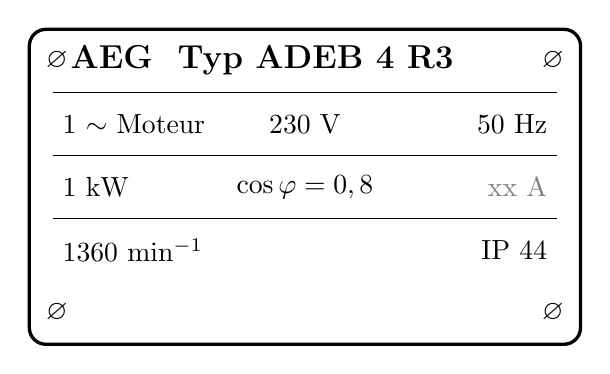
\begin{tikzpicture}
		\draw[rounded corners=6pt, very thick] (0,0) rectangle (7,4);
		\node[anchor=west, font=\bfseries\large] at (0.4,3.6) {AEG \ Typ ADEB 4 R3};
		\draw (0.3,3.2) -- (6.7,3.2);
		\node[anchor=west] at (0.3,2.8) {1 $\sim$ Moteur};
		\node at (3.5,2.8) {230 V};
		\node[anchor=east] at (6.7,2.8) {50 Hz};
		\draw (0.3,2.4) -- (6.7,2.4);
		\node[anchor=west] at (0.3,2.0) {1 kW};
		\node at (3.5,2.0) {$\cos\varphi = 0,8$};
		\node[anchor=east, text=gray] at (6.7,2.0) {xx A};
		\draw (0.3,1.6) -- (6.7,1.6);
		\node[anchor=west] at (0.3,1.2) {1360 min$^{-1}$};
		\node[anchor=east] at (6.7,1.2) {IP 44};
		\node at (0.35,3.6) {$\varnothing$};
		\node at (6.65,3.6) {$\varnothing$};
		\node at (0.35,0.4) {$\varnothing$};
		\node at (6.65,0.4) {$\varnothing$};
	\end{tikzpicture}
\end{center}


Sur quelle valeur de courant de déclenchement faut-il régler le disjoncteur de protection thermique du moteur ?

\begin{solution}


\begin{itemize}
    \item \textbf{Puissance utile ($P_2$) :} C'est la puissance mécanique fournie par l'arbre du moteur ($P_2 = \qty{1}{[kW]} = \qty{1000}{[W]}$).
    \item \textbf{Puissance absorbée ($P_1$) :} C'est la puissance électrique active réellement consommée sur le réseau. En raison du rendement $\eta = 0,83$ (\qty{83}{\%}), le moteur consomme plus de puissance qu'il n'en restitue : $P_1 = \dfrac{P_2}{\eta} \ \unit[]{[\watt]}$.
    \item \textbf{Courant nominal ($I_N$) :} C'est le courant alternatif monophasé qui circule dans le moteur en régime permanent à pleine charge : $P_1 = U \cdot I_N \cdot \cos\varphi \ \unit[]{[\watt]}$.
    \item \textbf{Réglage du disjoncteur thermique :} Le relais thermique (ou disjoncteur-moteur) est conçu pour protéger les enroulements contre les surcharges prolongées. Il doit être réglé exactement sur la valeur du courant nominal du moteur ($I_N$).
\end{itemize}


\textbf{Calcul de la puissance électrique active absorbée ($P_1$)}
\begin{align*}
P_1 &= \dfrac{P_2}{\eta} = \dfrac{\qty{1000}{}}{0,83} = \qty{1204,82}{[W]}
\end{align*}


\textbf{Calcul du courant nominal absorbé ($I_N$)}
\begin{align*}
P_1 &= U \cdot I_N \cdot \cos\varphi \ \unit[]{[\watt]}
\end{align*}
\begin{align*}
I_N &= \dfrac{P_1}{U \cdot \cos\varphi} = \dfrac{\qty{1204,82}{}}{\qty{230}{} \cdot 0,8} = \dfrac{1204,82}{184} = \qty{6,5479}{[A]} = \qty{6,55}{[A]}
\end{align*}


\textbf{Réglage du disjoncteur de protection thermique}
La protection thermique doit déclencher si le courant dépasse la valeur nominale admissible par les bobinages. Le courant de déclenchement du relais thermique doit donc être réglé sur :
\begin{align*}
I_N &= \qty{6,55}{[A]}
\end{align*}

Il faut régler le déclencheur thermique du disjoncteur-moteur sur \qty{6,55}{[A]} (ou \qty{6,5}{[A]} selon la graduation du cadran).

\begin{verbatim}
% Télécharger OCTAVE depuis https://wiki.octave.org/Using_Octave et l'installer
% Puis copier-coller le code dans OCTAVE

% Données de la plaque signalétique du moteur monophasé
P2_kW = 1.0;         % Puissance utile mécanique [kW]
P2 = P2_kW * 1000;   % Puissance utile [W]
U = 230;             % Tension alternative monophasée [V]
f = 50;              % Fréquence du réseau [Hz]
cos_phi = 0.8;       % Facteur de puissance
eta = 0.83;          % Rendement du moteur (83%)

% 1. Calcul de la puissance active électrique absorbée P1
P1 = P2 / eta;
printf("Puissance active absorbée : P1 = %.2f [W] (soit %.4f [kW])\n", P1, P1/1000);

% 2. Calcul du courant nominal absorbé I_N
I_N = P1 / (U * cos_phi);
printf("Courant nominal absorbé : I_N = %.4f [A]\n", I_N);

% 3. Valeur de réglage du disjoncteur thermique
I_reglage = I_N;
printf("Valeur de réglage de la protection thermique : I_réglage = %.2f [A]\n", I_reglage);
\end{verbatim}
\end{solution}
\end{questions}
\end{document}